
\chapter{Context and Computation Model}

In this part of the work, we will start by going over the general context of this problem and will take the opportunity to highlight the key factors of this kind of issues in order to propose solutions or, at least, try to resolve them. We will them follow by giving a brief summary of the numerous computation models related to parallelism to arrive at those more adapted to the representation of graphic cards\index{Graphics cards}. We will then give a high level explanation of how graphics cards\index{Graphics cards} work, their associated terminology and the issues that are intrinsically linked to them.

\section{General context}

Moore's law continues to be observed as a result of the various improvements both in the transistor, by a reduction of its size, and in the architecture, with increasingly complex realizations, which improve the computational power-energy ratio. Nevertheless, we see that it is increasingly difficult to stand up to different physical barriers~\cite{markov2014limits}.
One solution to this problem is the multiplication of computation units, among others such as quantum computers, 3D layering, new materials or photo-electronics. It can bypass the Pollack's Rule\footnote{Performance increase due to microarchitecture advances is roughly proportional to the square root of the increase in complexity~\cite{borkar2011future}.} to provide better yields. But that's not the only and single advantage:

The necessary computational power can be adjusted as best as possible (decrease the frequency or switch off the unit). This helps to balance the workload and distribute heat more evenly. This can also offer more resiliency, easier design and more robust architecture, less prone to bugs.

However, this flexibility is paid for by smaller and therefore less efficient individual computation units. This means that more parallelization is needed to achieve the same results, leading to communication problems for memory access and message transmission~\cite{borkar2011future}. It becomes all the more important to be able to offer algorithms that can run as independently as possible in order to take full advantage of all the parallelism offered.

Then comes Amdahl's law, which presents a very defeatist observation on the parallelism capacity of algorithms and their relative speed-up, the quantity of sequential part of the algorithms limits very strongly the theoretical maximum possible speed-up; or Gustafson's law, which wants to be more optimistic, by pointing out that the increase in computational power will also make it possible to respond to problems of greater size. In the following equations, $S$ represents the theoretical speedup in latency of the execution of the whole task, $p$ is the percentage of the execution workload which can me made parallel, $n$ the number of elements which can run in parallel and $s$ is the latency acceleration of the execution of the part of the task benefiting from the improvement of the system resources.

\vspace{15pt}

  \begin{minipage}[b]{0.35\linewidth}\centering
    $ S(n) = \frac{1}{(1 - p) + \frac{p}{n}} $ \\
    \vspace{15pt}
    Amdhal's law \\
  \end{minipage}\hfill
  \begin{minipage}[b]{0.55\linewidth}\centering
    $ S(n) = 1 - p + sp $ \\
    \vspace{15pt}
    Gustafson's law \\
  \end{minipage}
  
\vspace{15pt}

It is within this framework that we have sought to develop a data structure by adapting it to the context of graphic cards\index{Graphics cards}. This structure allows classic operations that appear in many algorithms and presents very interesting theoretical and technical characteristics. It also seeks to study a new way, that of using primitive elements of parallelism together in order to respond to the same problem and thus benefit from the additional computational power offered by such a practice.

The problem can be summarized as follows: we have new hardware with a very simplified architecture that offers massive parallelism. We therefore want to make the most of the available performance by exploiting both these new architectures and the very large number of processors. It should be noted that these devices also propose very specific notions to which it is necessary to pay attention.


\section{Model of computation}

Consequently, people began to look at how to parallelize algorithms and compare them through computational models to determine which ones performed best. The notions of complexity have been adapted to this new context and we have seen the emergence of many algorithms often presenting very elegant solutions. In this section, we will give a quick review of different models of computation which exist to compute the complexity of algorithms on parallel systems. There are countless of them with as many variations, we will limit ourselves to a ``canonical'' subset, the most famous ones and that will lead us to a particular computation model.

% Cache oblivious ? http://repository.cmu.edu/cgi/viewcontent.cgi?article=1104&context=compsci

% Interesting
% https://pdfs.semanticscholar.org/1417/c585009393cc2b45a38939a5e818738c62ea.pdf
% http://citeseerx.ist.psu.edu/viewdoc/download?doi=10.1.1.958.9741&rep=rep1&type=pdf

\subsection{PRAM}

This model was introduced in 1978 by S. Fortune and J. Wyllie~\cite{fortune1978parallelism,wyllie1979complexity}. They knew that we could not keep increasing performances of computers forever and therefore that one solution to this problem was to introduce parallelism in the computations. But, at that time, not many tried to determine what was the theoretical power of such machines.

The parallel random access machine (PRAM) can really be seen as an extension of the classical RAM model~\cite{cook1972time}. It describes an unbounded set of processors, with an infinite global memory and a set of input registers. Each processor has its own accumular, unbounded local memory, program counter and a flag which indicates whether or not the processor is running; there are also a list basic of instructions (load, store, add, jump, read) and some specific (fork and halt). The idea was to remain relatively close to the programming languages of the time while presenting a certain abstraction necessary to calculate the complexity of the various algorithms.

Its main specifities are the fork instruction, which initializes an inactive processor to start at a label, and the halt to stop running, other instructions are assimilated to the assembler's expression capacities. Traditionally, several processors are allowed to read simultaneously the same data but only one can write at a time on a specific cell; this assumption is often supported by the majority of materials designed as MIMD and is one of the possibilities offered by the model which can propose exclusivity or concurrency as well on the readings as on the writings since each instruction is executed in a cycle of three phases: a read (if any), a computation and a write (if any).

But most importantly, it defines classes of complexity where execution is determined on termination of the first processor. Hence, the time to accept an input is the minimum over all the computations from the first processor. Therefore, deterministic and non deterministic $T(n)$-TIME-PRAM classes are classically defined, some equivalences were also proven: $T(n)$-TIME-PRAM = $T(n)$-SPACE or N-$cT(n)$-TIME-PRAM = N-$2^{cT(n)}$-TIME (for $T(n) \geqslant \log(n)$)~\cite{fortune1978parallelism}.

For the first theorem, one should observe that the number of machine configurations in $T(n)$ algorithm is bounded by $2^{dT(n)}$. Then the equivalence is described as follow, the first processor is able to launch $2^{dT(n)}$ processes in $O(T(n))$, each holding a different number representing one configuration. They all decode their given configuration, compute the next one and encode it. Finally, to determine if the word is accepted from the initial configuration, it is sufficient for each processor to search for the successor configuration of the successor iteratively until we reach the termination state from the initial one (path-doubling strategy); all these operations can be performed in $O(T(N))$.

For the second, a similar argument can be used, each processor can guess one symbol of computation. The first $n$ processors check initial tape configuration, the others check that the symbol they consider corresponds well to that of the transition from the previous configuration and neighboring symbols. The latest processors must also verify that the state is accepting.

Many theoretical results on the bounds of algorithms were also obtained on models with slight variations in comparison to the original one~\cite{karp1988survey}. However, this model has some characteristics that make it unrealistic in practice. Indeed, there is no limit on the number of processors available on the machine. All basic operations are in constant time while some are obviously slower than others. Each processor can access any data and from anywhere, there is no difference between shared and distributed memory. Resource access management is simply ignored, there are no data contentions for instance. But it has the advantage of offering a working environment close to the mental conception of the problem.

\subsection{BSP}

Bulk Synchronous Parallel (BSP) was introduced in the late eighties by L. Valiant~\cite{valiant1990bridging}. It was designed to lie inbetween hardware and programming models, in the same way that the von Neumann machine is comparable to the Turing machine. This computer consists of three parts: \textit{components} able to perform processing (asynchronously) and memory operations, a \textit{router} which dispatchs the messages between pairs and a primitive (like a barrier) which allows synchronisation of all or only a subset of processors. This aims to symbolize the three main steps involved in any parallel algorithm, concurrent computing, communication and synchronization. This model thus makes it possible to represent other aspects which intervene in this type of algorithm and does not concentrate only on the computational complexity of the problem.

A computation, in this model, is described as a sequence of \textit{supersteps}. Each superstep is divided into three stages, a first where each component is allocated a task consisting of some local computation, then a communication phase is realized in order to propagate the results thanks to message transmissions and (implicitly) message arrivals from other components. Finally, after each period of $L$ time units, a global check is made to determine whether the system managed to accomplish the work within the allotted time. If it has, the machine can proceed the next superstep. Otherwirse, a new period is allocated to terminate the current superstep. Those $L$ units of time are called \textit{periodicity} and can be controlled at runtime. The lower bounds are set by the material capacities while the upper ones are rather software, by design, and related to the granularity of the solution since to achieve the optimal processor utilization, in each superstep, each processor should be assigned a task of approximately $L$ steps.

Some constants are defined like the communication bandwidth, the size of the local memory, the number of local operations per period or the maximal number of messages per superstep; some considerations about timings and relative proportions are also established. Hence, the cost of an algorithm is defined as the sum of three terms, the cost of the longest running local computation, the cost of communication inbetween processes and the cost of the synchronisation barrier (latency) at the end of the superstep. Each of them being summed on the number of supersteps needed to solve the problem.

The model knew many variations on the same theme and was recently updated to include several layers of cache\index{Cache} and the notion of optimality without paying attention about the parameters, also known as \textit{oblivious}~\cite{valiant2011bridging}.

Note that the MapReduce model, introduced by Google in 2004~\cite{dean2008mapreduce}, is based on similar concepts and can be reduced to it~\cite{senger2016bsp}. It focuses mainly on problems related to Big Data and provides a more practical framework. The data is first loaded and distributed between the different processors. Each then applies a function \textit{map} that transforms the local data and writes the result into a temporary storage area. The results are then redistributed on the basis of keys, also produced during the map operation, so that all the data belonging to the same key are sent to the same processor, this is the big \textit{shuffle}. Finally, each processor reworks those new data by key in parallel, \textit{reduce}. There are thus two ``BSP supersteps'' in one in this model.

\begin{figure}[!ht]
\centering
\begin{minipage}{.5\textwidth}
  \centering
  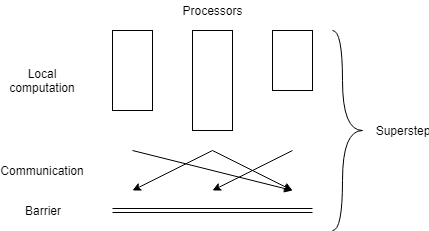
\includegraphics[width=0.9\linewidth]{Chapters/GPU/BSP.png}
  \captionof{figure}{BSP}
  \label{fig:BSP}
\end{minipage}%
\begin{minipage}{.5\textwidth}
  \centering
  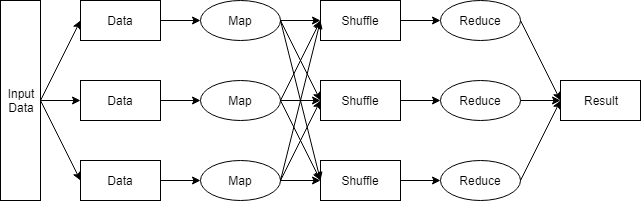
\includegraphics[width=0.9\linewidth]{Chapters/GPU/MapReduce.png}
  \captionof{figure}{MapReduce}
  \label{fig:MapReduce}
\end{minipage}
\end{figure}

\subsection{LogP}

The canonical PRAM model, even though it proposes nice theoretical results, is not representative of real-life computers due to its zero communication delay, synchronism among all the execution steps or infinite bandwidth. On the opposite, BSP may represent a too large variety of machines whereas we see a convergence towards a same architecture for distributed computing: many complete computers connected by a communication network. LogP model proposed in 1993 by Culler and al.~\cite{culler1993logp} tried to take place inbetween those two models. It focuses on high level abstraction of the machine and target essentially communication (message-passing style).

Some parameters are defined such as an upper bound on latency $L$ incurred by sending a message from a source to a destination, an overhead $o$ linked to the inactivity of the processor while sending or receiving messages, a gap $g$ defined as the minimum time between two consecutive messages and $P$ the number of processes. This model assumes that the network has a finite capacity ($\frac{L}{g}$ messages from any one processor to any other), asynchronous communication and messages are expected to be small, 

The BSP and LogP models focus on different concepts, they do not aim at the same purpose. For BSP, barrier synchronisation and routing of messages are primitives and is much likely used to design algorithm. Whereas LogP proposes a better control of resources with loose synchronisation. But, more importantly, they propose a comparable power of computation to design algorithms and so BSP tends to be easier to manage and provides a more convenient programming abstraction~\cite{bilardi1999bsp}.

\subsection{PDM}

Aggarwal and Vitter introduced in 1988~\cite{aggarwal1988input} the external memory model (EM) or disk access machine (DAM) which counts the number of block\index{Block} I/Os to and from an external source of memory. The idea was that, at the time, the memories were too small to hold the entire dataset, so it was necessary to regularly fetch the data from an external source (i.e. magnetic tapes). EM algorithms explicitly control data placement and transfer to reduce the number of data queries to be made and their inherent slowness, disk accesses are 1 million times slower than the execution of one instruction on modern computer.

Once the desired data location has been found on the tape, accessing neighboring data is very simple. And since we also tend to want to access information located nearby (as in the case of a for loop), it can be interesting to amortize the relatively long initial delay to access a data by transferring a large contiguous group of data items at a time. We use the term \textit{block}\index{Block} to refer to the amount of data transferred to or from one disk in a single I/O operation.

With an analoguous spirit, Vitter and Shriver introduced the parallel disk model (PDM) which combines the notion of locality of references and the parallel accesses. All the processors read in main memories and many blocks\index{Block} of data can be swapped from different disks in parallel. Those models really captured the essential notions to exploit the locality as well as the load balancing to deserve our programs. Many results were achieved through these models and Vitter compiled many algorithms, with their analysis and their associated data structure in one interesting book~\cite{vitter2008algorithms}. Interests about technical difficulties and their practical solutions are also suggested but the main interest relies on sequential algorithms.

PDM uses the following main parameters: $N$ the problem size, $M$ the internal memory\index{Cache} size, $B$ the block\index{Block} transfer size, $D$ the number of independent disk drives and $P$ the number of processors.

Such that, in a single I/O, each of the $D$ disks can simultaneously transfer a block\index{Block} of $B$ contiguous data items. The data needs to be placed in internal memory $M$\index{Cache} in order to be able to perform the appropriate processing. The parallelism proposed by this model must be considered more as a weaker form, since the memory is distributed, each processor has its own internal memory and attached set of disks. It could be seen more as $P$ copies of EM machines.

\subsection{PEM}

As the external memory model (and its brother ``cache-oblivious''\index{Cache oblivious}) brings the notion of cache\index{Cache} and memory transfers to the RAM model, PEM realizes the same idea but with PRAM model. Bender et al., tried in 2005~\cite{bender2005concurrent}, to combine the notion of cache-oblivious\index{Cache oblivious} with parallelism but were more focused on one specific data structure, a B-tree\index{B-tree}. The underlying idea was that the cache\index{Cache} can be viewed as a bounded memory which can read or write from an external and global memory.

Finally, L. Arge, M. T. Goodrich, M. Nelson and N. Sitchinava, in 2008~\cite{arge2008fundamental}, came up with Parallel External Memory (PEM) model. It can be viewed as a single-disk external memory shared by several processes all owning a private cache\index{Cache}.

This model differs fundamentally from the previous model of computation as it keeps some shared memory. There is only one external data source that can be accessed by any processor. Nonetheless, each processor has its own internal memory, which introduces thus problems related to concurrency and data consistency. Be aware that no mechanism of synchronisation or communication among processors are provided and further extensions exist to treat the concurrent reads and writes.

It also makes the assumption that the performances are bounded by the I/O and its intrinsic latency. This model is defined by few parameters, $N$ the problem size, $P$ the number of processors, $M$ the cache\index{Cache} size and $B$ the block\index{Block} size. So the parameters are essentially the same than the previous one, the only difference is that there is only one disk.

\begin{figure}[!htb]
    \centering
    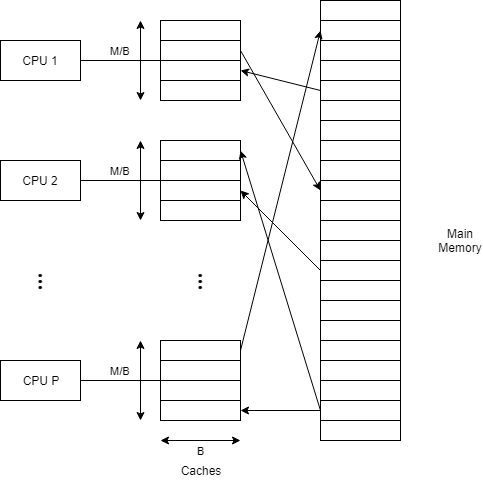
\includegraphics[width=0.5\linewidth]{Chapters/GPU/PEM.png} 
    \caption{PEM model}
\end{figure}

\subsection{TMM}

Threaded Many-core Memory model of computation was described in 2014 by L. Ma et al.~\cite{ma2014memory}, it wants to stay relatively close to the architecture found in GPUs. This model explicitly models the large number of threads per processor and the memory latency to slow memory. It mainly proposes finite constraints on the execution (on the contrary of the model PRAM which does not bound the number of processors) while not targeting a precise hardware or trying to calibrate the performance model.

It is defined by six parameters linked to I/O complexity: the time for a global memory access, the number of processors, the number of elements transfered per block\index{Block}, the size of the local memory\index{Cache} attached per group, the number of cores per group and the maximal number of threads per core.

As well as other parameters which are determined by the algorithm and more in relation to time complexity and PRAM notions. We find the total amount of work and per thread, the number of threads per core and the amount of memory space required per each thread. It is one of the many models which exist, but it offers both time and I/O complexity analysis. One can therefore expect stronger optimality criteria, if the algorithm is both optimal in time and in I/Os.

\subsection{Quantitative model}

More recently, people try to model the architecture of the GPU and their relative operations more accurately~\cite{baghsorkhi2010adaptive,hong2009analytical}. The idea was to find out bottlenecks in the implementation through static analysis and to provide tips for the developpers. Highlight operations that are supposed to be slow such that the user can be able to optimize them; or propose metrics to guide compiler optimization passes.

Hence, they go much more further in the concepts which intervene in the modelisation and provide more adhoc comparisons of implementations with the relative timing of each instruction. They represent the code through a work flow graph which feeds the computation and memory pipelines. Warps, SIMD instructions\index{SIMT} and other factors (like the number of threads, the block size, the cache size...) which may come into account while tuning performances are also taken into consideration. Considerations for which more explanation will be provided in the following section$^{[\ref{GPU}]}$.



\section{GPU}\label{GPU}

Graphics processor units (GPU)\index{Graphics cards} were specialized pieces of hardware mainly dedicated to the treatment of images and matrices application. Now, they provide massive parallelism with low power consumption and which can be used for many algorithms. It is also known by its acronym; GPGPU (General-Purpose computing on Graphics Processing Units). The goal of GPU computing is to achieve the highest performance for data-parallel problems through a massive parallel algorithm.

In the early 2000s, processing units were built upon a programmable architecture, permitting to the user to define their own running execution (the so-called ``shaders''). People tried to adapt the graphical notions to more classical and scientific problems but it was difficult to realize from a technical point of view. Little by little, the idea to use GPUs thanks to their low power consumption, high parallelism and low cost led people to try to overcome these difficulties. Hence, some first solutions were proposed with a more flexible programming language~\cite{buck2004brook}.

However, the way the GPUs work differ fundamentally from the CPUs. Indeed, the structure is inherently massively parallel, with no classical notion of stack (and thus no function stack), and with a different notion of memory layout (\textit{coarse-grained data parallelism}), hence cache\index{Cache}. Designing GPU-efficient algorithms is therefore challenging and requires some adaptation. Nevertheless, the architecture provides natural independence in the number of physical processing units available or how execution order of threads is scheduled.

In order to execute a program capable of running on a graphics card\index{Graphics cards}, a \textit{kernel}, it is required to write API-compliant code; there are two main API, namely, CUDA and OpenCL (which will disappear to be integrated into Vulkan). To ``simplify'', these use two different terminologies, we will use mostly the terminology that accompanies the CUDA environment in the rest of this work but in this part, we will present both.

A \textit{thread} or \textit{work-item} represents one hardware thread of execution, a sequence of instructions. But these are, in practice, executed in groups, called \textit{warp} or \textit{subgroup}, typically of size 32 and who can directly communicate with each other. The underlying idea is that we want to execute multiple threads, sharing the same code, at the same time for parallelism. Thus, as soon as we decode an instruction, we are able to execute it on all of them at once. This technique is called Single Instruction Multiple Thread (SIMT)\index{SIMT}.

A \textit{block} or \textit{group} is formed from a set of warps. This unit of parallelism contains, depending on the hardware, up to 2048 threads or 64 warps that can exchange data through shared memory. They are also attached to a \textit{streaming multiprocessor} which plays the equivalent of a core and which schedules the execution of these warps on the computing unit. Finally, as we have several streaming multiprocessors at our disposal, we can run several blocks at a time in parallel. This set of blocks and threads is called \textit{grid} or \textit{workspace} and designates the whole collection of threads to execute. A grid can therefore represent several thousands of threads and is assigned to a kernel.

The main purpose of these notions is to allow higher abstraction for better scaling without considering technical details about scheduling or their quantities. The architecture is also designed to hide latency, whenever one warp has to wait (the result of a memory access or a long operation), another can take its place. A very large amount of threads is therefore beneficial to this type of architecture, since they are very light and can be easily swapped.

\begin{figure}[!ht]
\centering
\begin{minipage}{.5\textwidth}
  \centering
  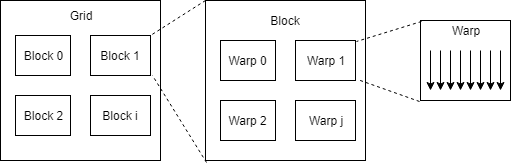
\includegraphics[width=0.9\linewidth]{Chapters/GPU/ThreadHierarchy.png}
  \captionof{figure}{Thread hierarchy}
  \label{fig:BSP}
\end{minipage}%
\begin{minipage}{.5\textwidth}
  \centering
  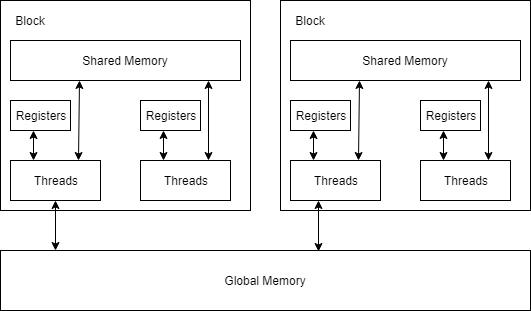
\includegraphics[width=0.9\linewidth]{Chapters/GPU/MemoryHierarchy.png}
  \captionof{figure}{Memory hierarchy}
  \label{fig:MapReduce}
\end{minipage}
\end{figure}

%\begin{figure}[!htb]
%    \centering
%    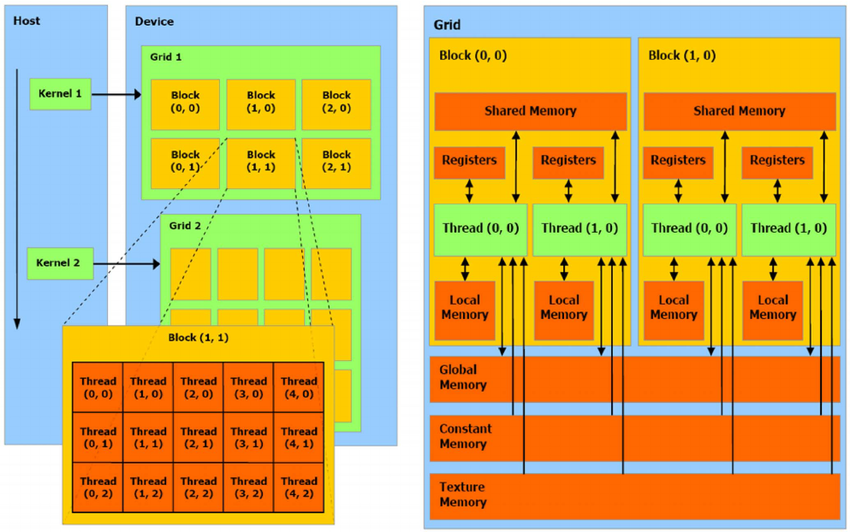
\includegraphics[width=\linewidth]{Chapters/GPU/CUDA-architecture.png} 
%    \caption{Schematization of GPU architecture - image extracted from Nobile et al.~\cite{nobile2014cutauleaping}, doi:10.1371/journal.pone.0091963.g001}
%\end{figure}

Beyond the thread hierarchy, GPU memory is organized into three ``main'' levels: global, shared/local and private with different sizes and speeds. The global memory is accessible from any thread in the grid, this is the equivalent of our external data source. It typically contains several GB of data and has a bandwidth of over 100GB/s. Shared memory is accessible only by threads being located within a same block, and thus linked to a streaming multiprocessor. It is much smaller, about 32KB, but is incredibly fast, it can peak up to 1300GB/s. Finally, private memory is only accessible within one warp. Its size and speed are not fixed since they can be located in different places, either in registers, shared or global memory, but for communication operations between members of the same warp, we can expect up to 7500GB/s.

Memory is also explicitly managed instead of what we found in an implicit cache\index{Cache} system (like a CPU). This aims to offer the possibility to take advantage of those for our particular problem through caching and prefetching policies which can be specifically designed according to algorithmic or application needs. At the same time, its handling is crucial to obtain the best performance possible~\cite{ueng2008cuda}. Most of the specific features proposed by those API are only dedicated to this aspect.

The programming work-flow of GPU computing is also different. It defines a host-device relationship between the CPU and GPU. This helps to take advantage of heterogenous computation. The principle is simple, a host program uploads the problem into the device (GPU memory), and then invokes a kernel passing the different parameters of the problem: the number of threads per block as well as the number of blocks, and the arguments of the program. The host program can either work in a synchronous or asynchronous manner, depending if the result from the GPU is currently needed for the next step or not. When the kernel has finished in the GPU, the result data is copied back from device to host~\cite{stone2010opencl}.

In practice, the essential difference with traditional programming is parallelism management. It is necessary to aim that the processings are the same for all threads. Only, it is not possible in all cases, either because the problem does not lend itself to it, or because the algorithm is not sufficiently adapted. Parallelism can then be controlled more precisely, first by dealing with the problem in blocks and if necessary by warps. By trying each time that there is a minimum of divergence between these different levels of parallelism.

The divergence in the computations is one of the biggest issues. Since an instruction is applied to the entire warp, this implies that each execution flow must be performed one after the other when there is a branching, with a mask indicating whether the results should be conserved or not. If everyone takes the same path, there are no such problems. The more branchings the code has, the slower it will be.

With this crucial aspect, care must be taken to consume the best available resources (registers or memories) in order to allow maximum parallelism and benefit from the locality of the data.

\subsection{Hardware considerations}

Many considerations come into account while implementing algorithms on GPU and which can have significant impact on the performances that will be achieved. We will try to remain as abstract as possible on problems that are highly technical. We must therefore be attentive, when programming, to various concepts. Achieving the maximum possible performance from these tools is often very difficult and it is best to keep different elements in mind. Algorithms can also be designed to rely on these underlying ideas.

\subsubsection{Coalesced\index{Coalesced} memory}

This notion refers to the ideal scenario of memory accesses where consecutive threads access to consecutive chunks of data. This access pattern helps the data prefetching and, thus, to increase the memory bandwidth, making the implementation more efficient. This also corresponds to the notion of blocks\index{Block} found in the external memory computation model. On the other side, irregular access patterns will lead to reduced performances~\cite{baskaran2008optimizing}.

Note that the term coalesced\index{Coalesced} is more specifically used when the memory address is aligned on a multiple of the entire cache\index{Cache} line and each thread accesses the element associated with its bank (small independant memory cell), the one linked to its identifier (more practically, this corresponds thus to the case mem[cache line size * k + thread identifier]). We will return to these notions in more details in a forthcoming chapter$^{[\ref{Accesses}]}$.

\subsubsection{Bank conflict}

% http://gpgpu.org/wp/wp-content/uploads/2013/09/08-opti-smem-instr.pdf

To speed up data access, shared memory is divided into small contiguous memory areas (about 4 bytes) called \textit{bank}. These units guarantee extremely fast accesses at the price of being able to process only one request at a time. So we also have to be cautious about \textit{bank conflicts} which occur when multiple threads attempt to access elements inside the same shared memory bank, those are then serialized leading to poor performances. The hardware splits a memory request with bank conflicts into as many separate conflict-free requests as necessary, decreasing throughput by a factor equal to the number of separate memory requests. The latest hardware versions are capable of broadcasting the data if they are located inside the same word, but accessing different words remains a problem~\cite{micikevicius2013performance}.

\subsubsection{Thread coarsening}

The granularity of the program can really affect the performances. Fine-grained tasks cause greater parallelism and therefore increases the speed-up, however more synchronization or scheduling strategies are also needed, which can have a negative impact on the performance. On the other hand, coarse-grained tasks have lower communication overhead, but often cause a load imbalance. It also allows to reuse same computation among the several tasks in unified manner or to reduce the overhead linked to the latency of the threads scheduling. Thread coarsening consists essentially to reduce the granularity of the algorithm to increase the amount of work per thread. Finding the good granularity is thus a really experimental tuning and the value of such process is usually limited due to the constantly reducing time required to launch a new kernel, schedule new warps or thanks to hardware improvements.

\subsubsection{Shared memory and caching}

The SIMT multiprocessors have fast private memory shared by all its cooperating threads. And threads are also layered in blocks which can all access to a share and common memory among all of them. Those two levels of cache\index{Cache} memory are orders of magnitude faster than the global device memory and thus can be exploided for peak performances.

\subsubsection{Padding}

Padding is the act to adjust the problem size on the level of the data to get a multiple of the block sizes. There is no more edge corner when considering the last elements of the problems. They fit tightly in the grid and thus require no more special treatment. Of course, the extra dummy data must not affect the original results. With padding, one can avoid putting conditional
statements in the kernel that would lead to unnecessary branching~\cite{navarro2014survey}.

\subsubsection{Branching}

Branching occurs when there are conditional statements in the kernel, both branches are then executed sequentially\index{Sequential}. It has a negative impact in performance and should be avoided whenever possible. The reason why branching occurs is because all threads within a warp execute in a lock-step mode and will run completely in parallel only if they follow the same execution path in the kernel code (SIMT\index{SIMT} computation); the result is thus discarded for the threads who did not take that path. If any conditional statement breaks the execution into two or more paths, then the paths are executed sequentially. Conditionals can be safely used if one can guarantee that the program will follow the same execution path for a whole warp. Additionally, we can use some logical operators which cause no branching and can be used to make disappear simple conditionals~\cite{harris2007parallel}.

\subsubsection{Memory use vs parallelism}

Finally, we said that the architecture conceptually allows an abstraction between the number of blocks and threads we launch and the real hardware capabilities. However, in practice, this is not totally the case, resources are scarce. The shared memory is very small (32KB) and can be shared by thousand threads; there are also only 256 registers but these condition the number of warps executable simultaneously on the same streaming multiprocessor, if we want to have in practice a thousand threads active, we should consume only 32 of them. Moreover, the more active threads there are, the more memory requests will be made and with them the number of cache\index{Cache} evictions. It is thus a real trade-off which must be carried out between the number of threads and blocks which one wants to execute and the resources which one can use.



\section{Design}

Designing an algorithm is not a trivial task; even more, in case of parallelism. There are some strategies to help us to create efficient and parallel algorithms but there are also some considerations to take into account. In 1995, Foster~\cite{foster1995designing} identified four key components to design many algorithms.

\subsection{Partitioning}

The first idea which comes to mind when trying to solve some parallel problem is to find out how to split it into several subproblems. The goal is thus to identify whether it is possible to partition either at the level of the data or at the level of the tasks. If the subproblems can work on different data at the same time, we tend to say that there is data-parallelism. On the other hand, when the tasks do not conflict each other, we use the notion of task-parallelism. Those two big families are represented through a large variety of problems. But, data-parallelism seems more in adequation with data-driven programs, like physics simulation or data science. Whereas, task-parallelism arises more often in algorithmetical problems such as graph traversals or flow notions.

\subsection{Communication}

When the method of partitioning has been determined, we still need to consider the communication. This is often divided into two categories: the local and the global communication. Local communation appears when subproblems can easily communicate with their neighbours to continue their work. Global communication, on the opposite, involves broadcast to be able to make the next step. In this phase, all the problems linked to communication and concurrency need to be handled through different and classical methods as critical sections or barriers to ensure consistency among the workers and reliability in the results.

\subsection{Agglomeration}

Even though, we have nice partitioning with small communication requirements, there may be some imbalances in the resulting computations and it would be nice if we could rebalance the problem while running it. This aspect related to the granularity of the problem. Fine-grained divide the problem into a huge number of jobs but with a lot of communication; coarse-grained perform less jobs but with larger tasks. This is a trade-off between parallelism and communication. Agglomeration seeks thus to find the best compromise of granularity while taking into account the final implementation.

\subsection{Mapping}

With the recent advances in the hardware and algorithmic considerations, it may be interesting to consider how the agglomerations will be mapped to computational processors. The way those are distributed among the cores and their relative order can have significant impact on the performances of the final implementation of the algorithm. We want, of course, to have a direct mapping or, at least, the simplest method to avoid higher hardware complexity and overhead. But, this may lead to counter techniques which enhance balancing. This category really became prominent with distributed memory and GPU computing where exploiting hardware may lead to signifcant improvements.

It is therefore interesting to offer this aspect to developers so that they can choose what suits them best and this results in the consideration or not of notions of warps, blocks or grids in algorithms. Knowing which primitives we are working on allows simplifications that can make the code much more efficient.

\subsection{Brent's scheduling principle}

{
\setstretch{0.95}
When we speak of parallelism, the notion of Brent's Scheduling Principle is often mentioned, it synthesizes a logical observation that appears when we study parallel algorithms in a more algorithmic and complexity-related framework.

Some algorithms are said to be time optimal if the number of steps in parallel program is equal to the number of steps in the best sequential algorithm. One should remark that there are two main way to associate the complexity in parallel algorithms:

\begin{itemize}
    \item Either, we consider the time complexity of a parallel algorithm as the number of steps taken by each processor, denoted by $S(N)$ and called \textit{span}.
    \item Either, we study the complexity of the whole task as the total number of operations the algorithm performed by every processors, denoted by $W(N)$ and called \textit{work}.
\end{itemize}

If a parallel algorithm runs in $S(N)$ and uses a total of $W(N)$ operations, it can be simulated on a $P$-processor PRAM
in no more than $T_{C}(N, P) = W(N)/P + S(N)$ parallel steps. This is known as Brent's Scheduling Principle~\cite{gibbons1989more} but, this principle does not apply to PEM model of computation. Since, if we apply the same idea with a round-robin simulation of the processors, this would lead, in worst-case, to $\Theta(\frac{PM}{B})$ factor due to the fact that we need to load the entire memory of each processor to simulate it. There is no equivalent theorem in this framework, the closest states that a PRAM algorithm in time $T(N)$ of $N$ processors and $O(N)$ space can be simulated in $O(T(N) \text{ sort}(N))$ I/Os~\cite{chiang1995external}.

The whole point of Brent's Scheduling Principle is that it provides equivalence between parallel and sequential programs. This mainly means that if an algorithm has a better complexity in the parallel framework, then there exists a sequential program equivalent with the same work complexity since we could easily simulate the parallel one.

}
